%%This is a very basic article template.
%%There is just one section and two subsections.
\documentclass{article}

% This file includes a set of standard packages used to configure latex

\usepackage[utf8x]{inputenc}
\usepackage[T1]{fontenc}
%\usepackage{mathptmx} % Use Times Font
\usepackage{cmbright} % Use Sans-Serif Font
\usepackage[pdftex]{graphicx} % Required for including pictures
\usepackage[pdftex,linkcolor=black,pdfborder={0 0 0}]{hyperref} % Format links for pdf
\usepackage{calc} % To reset the counter in the document after title page
\usepackage{enumitem} % Includes lists
\usepackage{subfigure}
\usepackage{fullpage}
\usepackage[all]{nowidow} % Tries to remove widows
\usepackage[protrusion=true,expansion=false]{microtype} % Improves typography, load after fontpackage is selected
\usepackage{amsmath}     % For mathematical equations
\usepackage{amsfonts}     % For mathematical equations
\usepackage{booktabs}    % For table formatting

% Comment out these lines to disable default bold
\renewcommand{\seriesdefault}{\bfdefault}
\mathversion{bold}

\usepackage{amssymb} %maths
\usepackage{amsmath} %maths
%\usepackage[utf8]{inputenc} %useful to type directly diacritic characters
\usepackage{bm}
\usepackage{siunitx}

% Functions
\newcommand{\Func}[2]{\mathbf{#1}\left[#2\right]}

% Integration
\newcommand{\defint}[3]{\int_{#1}{#2}\bm\mathrm{d}{#3}}
\newcommand{\indefint}[2]{\int{#1}\mathbf{d}{\bm #2}}

% Probability and random variables
\newcommand{\rv}[1]{\mathsf{#1}}
\newcommand{\prob}[1]{\mathrm{p}\left(#1\right)}
\newcommand{\ProbSet}[1]{\mathrm{P}\left\{#1\right\}}
\newcommand{\pdf}[1]{\bm{f\left(#1\right)}}
\newcommand{\E}[1]{\mathbb{E}\bm\left[#1\right]}
\newcommand{\dummyScalarX}{\bm{x}}
\newcommand{\dummyScalarXMean}{\bm{\hat{x}}}
\newcommand{\dummyScalarXErr}{\bm{\tilde{x}}}
\newcommand{\dummyScalarY}{\bm{y}}
\newcommand{\dummyScalarYMean}{\bm{\hat{y}}}
\newcommand{\dummyScalarYErr}{\bm{\tilde{y}}}

% Base definitions
\renewcommand{\Vec}[1]{\mathbf{#1}}
\newcommand{\VecHat}[1]{\hat{\mathbf{#1}}}
\newcommand{\VecTilde}[1]{\tilde{\mathbf{#1}}}
\newcommand{\VecTime}[2]{\Vec{#1}_{\bm{#2}}}
\newcommand{\VecTimeSup}[3]{\Vec{#1}_{\bm{#3}}^{\bm{#2}}}
\newcommand{\VecHatTime}[2]{\VecHat{#1}_{\bm{#2}}}
\newcommand{\VecHatTimeP}[3]{\VecHat{#1}^{\bm{#3}}_{\bm{#2}}}
\newcommand{\VecTildeTime}[2]{\VecTilde{#1}_{\bm{#2}}}
\newcommand{\VecTildeTimeT}[2]{\VecTilde{#1}^\top_{\bm{#2}}}
\newcommand{\VecTimeTranspose}[2]{\Vec{#1}^\top_{\bm{#2}}}
\newcommand{\VecDotTime}[2]{\dot{\Vec{#1}}_{#2}}

\newcommand{\Mat}[1]{\mathbf{#1}}
\newcommand{\MatT}[1]{\mathbf{#1}^\top}
\newcommand{\MatiTime}[2]{\mathbf{#1}^{\bm{-1}}_{\bm{#2}}}
\newcommand{\MatTime}[2]{\mathbf{#1}_{\bm{#2}}}
\newcommand{\MatTimeSup}[3]{\mathbf{#1}_{\bm{#3}}^{\bm{#2}}}
\newcommand{\MatTimeSupT}[3]{\mathbf{#1}_{\bm{#3}}^{\bm{#2}}{}^{\bm\top}}
\newcommand{\MatTimeT}[2]{\mathbf{#1}^\top_{\bm{#2}}}

% Gradients
\newcommand{\Grad}[1]{\boldsymbol{\nabla}{\Mat{#1}}}
\newcommand{\GradBy}[2]{\boldsymbol{\nabla}_{\bm{#2}}{\Mat{#1}}}
\newcommand{\GradT}[1]{\boldsymbol{\nabla}^\top{\Mat{#1}}}
\newcommand{\GradByT}[2]{\boldsymbol{\nabla}^\top_{\bm{#2}}{\Mat{#1}}}

% Statistics
\newcommand{\xmean}[1]{\VecHatTime{x}{#1}}

% Discrete-time state space equations
\newcommand{\DT}{\Delta{T}}
\renewcommand{\u}[1]{\VecTime{u}{#1}}
\newcommand{\U}[1]{\VecTime{U}{#1}}
\renewcommand{\v}[1]{\VecTime{v}{#1}}
\newcommand{\vp}[2]{\VecTime{v}{#2}^{#1}}
\newcommand{\vT}[1]{\VecTimeTranspose{v}{#1}}
\newcommand{\w}[1]{\VecTime{w}{#1}}
\newcommand{\wT}[1]{\VecTimeTranspose{w}{#1}}
\newcommand{\wt}[1]{\VecTimeTranspose{w}{#1}}
\renewcommand{\wp}[2]{\VecTimeSup{w}{#1}{#2}}
\newcommand{\x}[1]{\VecTime{x}{#1}}
\newcommand{\s}[1]{\VecTime{s}{#1}}
\newcommand{\zp}[2]{\VecTimeSup{z}{#1}{#2}}
\newcommand{\z}[1]{\VecTime{z}{#1}}
\newcommand{\Z}[1]{\VecTime{Z}{#1}}
\newcommand{\xp}{\Vec{x}^{\prime}}
\newcommand{\procModel}[1]{\mathbf{f}\left[#1\right]}
\newcommand{\obsModel}[1]{\mathbf{h}\left[#1\right]}
\newcommand{\invObsModel}[1]{\mathbf{g}\left[#1\right]}
\newcommand{\F}[1]{\VecTime{F}{#1}}
\newcommand{\Fp}[2]{\MatTimeSup{F}{#1}{#2}}
\newcommand{\FpT}[2]{\MatTimeSupT{F}{#1}{#2}}
\newcommand{\FT}[1]{\VecTimeTranspose{F}{#1}}
\renewcommand{\H}[1]{\VecTime{H}{#1}}
\newcommand{\HT}[1]{\MatTimeT{H}{#1}}
\newcommand{\Hp}[2]{\MatTimeSup{H}{#1}{#2}}
\newcommand{\B}[1]{\VecTime{B}{#1}}
\newcommand{\Bp}[2]{\MatTimeSup{B}{#1}{#2}}
\newcommand{\BpT}[2]{\MatTimeSupT{B}{#1}{#2}}

% Continuous time quantities
\newcommand{\xDot}[1]{\VecDotTime{x}{#1}}

\newcommand{\Q}[1]{\MatTime{Q}{#1}}
\newcommand{\Qp}[2]{\MatTimeSup{Q}{#1}{#2}}
\newcommand{\R}[1]{\MatTime{R}{#1}}
\newcommand{\Rp}[2]{\MatTimeSup{R}{#1}{#2}}


% Kalman filter


\newcommand{\xEst}[2]{\VecHatTime{x}{#1|#2}}
\newcommand{\var}[2]{\Mat{P}_{\bm{#1|#2}}}
\newcommand{\varP}[3]{\Mat{P}_{\bm{#2|#3}}^{\bm{#1}}}
\newcommand{\xErr}[2]{\VecTildeTime{x}{#1|#2}}
\newcommand{\xErrT}[2]{\VecTilde{x}^\top_{\bm{#1|#2}}}
\newcommand{\sErr}[2]{\VecTildeTime{s}{#1|#2}}
\newcommand{\sErrT}[2]{\VecTilde{s}^\top_{\bm{#1|#2}}}
\newcommand{\K}[2]{\MatTime{K}{#1|#2}}
\newcommand{\W}[2]{\MatTime{W}{#1|#2}}
\newcommand{\WT}[2]{\MatTimeT{W}{#1|#2}}
\renewcommand{\S}[2]{\MatTime{S}{#1|#2}}
\newcommand{\Si}[2]{\MatiTime{S}{#1|#2}}
\newcommand{\C}[2]{\MatTime{C}{#1|#2}}

\newcommand{\zEst}[2]{\VecHatTime{z}{#1|#2}}
\newcommand{\innov}[2]{\boldsymbol{\nu}_{\bm{#1|#2}}}
\newcommand{\innovT}[2]{\boldsymbol{\nu}^\top_{\bm{#1|#2}}}

% Particle filters
\newcommand{\xpart}[2]{\Vec{x}_{#2}^{[#1]}}
\newcommand{\wpart}[2]{w_{#2}^{[#1]}}




% SLAM

% System equations

\newcommand{\xSlam}[1]{\VecTime{s}{#1}}
\newcommand{\xPlat}[1]{\VecTime{x}{#1}}

\newcommand{\zSlam}[2]{\Vec{z}_{\bm{#2}}^{\bm{#1}}}
\newcommand{\wSlam}[2]{\Vec{w}_{\bm{#2}}^{\bm{#1}}}
\newcommand{\RSlam}[2]{\Mat{R}_{\bm{#2}}^{\bm{#1}}}
\newcommand{\islam}[2]{\bm{i}_{\bm{#2}}^{\bm{#1}}}
\newcommand{\mx}{\Vec{m}}
\newcommand{\lmx}[1]{\Vec{m}^{\bm{#1}}}
\newcommand{\lmxEst}[3]{\VecHatTime{m}{#2|#3}^{\bm{#1}}}
\newcommand{\lmxErr}[3]{\VecTildeTime{m}{#2|#3}^{\bm{#1}}}
\newcommand{\lmxErrT}[3]{\VecTildeTime{m}{#2|#3}^{\bm{#1},\top}}
\newcommand{\lmxx}[1]{\bm{x}^{\bm{#1}}}
\newcommand{\lmxy}[1]{\bm{y}^{\bm{#1}}}
\newcommand{\info}[1]{\mathbb{I}_{#1}}

\newcommand{\mEst}[2]{\VecHatTime{m}{#1|#2}}
\newcommand{\mErr}[2]{\VecTildeTime{m}{#1|#2}}
\newcommand{\mErrT}[2]{\VecTildeTimeT{m}{#1|#2}}
\newcommand{\mEstP}[3]{\VecHatTimeP{m}{\bm{#2|#3}}{\bm{#1}}}

\newcommand{\xSlamEst}[2]{\VecHatTime{s}{#1|#2}}
\newcommand{\xErrSlam}[2]{\xErr{#1}{#2}}
\newcommand{\xErrSlamT}[2]{\xErrT{#1}{#2}}
\newcommand{\varSlam}[2]{\varP{s}{#1}{#2}}
\newcommand{\vSlam}[1]{\vp{s}{#1}}

\newcommand{\xPlatEst}[2]{\VecHatTime{x}{#1|#2}}
\newcommand{\xPlatErr}[2]{\VecTildeTime{x}{#1|#2}}
\newcommand{\xPlatErrT}[2]{\VecTilde{x}^\top_{\bm{#1|#2}}}
\newcommand{\FPlat}[1]{\F{#1}}%\F|{\MatTimeSup{F}{\mathbf{x}}{#1}}
\newcommand{\FPlatT}[1]{\FT{#1}}%{\MatTimeSupT{F}{\mathbf{x}}{#1}}
\newcommand{\BPlat}[1]{\B{#1}}%{\MatTimeSup{B}{\mathbf{x}}{#1}}
\newcommand{\BPlatT}[1]{\F{#1}}%{\MatTimeSupT{B}{\mathbf{x}}{#1}}
\newcommand{\vPlat}[1]{\v{#1}}%{\vp{\mathbf{x}}{#1}}
\newcommand{\QPlat}[1]{\Q{#1}}%{\MatTimeSup{Q}{s}{#1}}
\newcommand{\varPlat}[2]{\varP{\mathbf{xx}}{#1}{#2}}
\newcommand{\HSlam}[1]{\MatTimeSup{H}{s}{#1}}
\newcommand{\HSlamT}[1]{\MatTimeSupT{H}{s}{#1}}


\newcommand{\xSlamPartialEst}[2]{\VecHatTimeP{s}{\bm{#1|#2}}{*}}
\newcommand{\lmxPartialEst}[3]{\VecHatTimeP{m}{\bm{#2|#3}}{*,#1}}
\newcommand{\xPlatPartialEst}[2]{\VecHatTimeP{x}{\bm{#1|#2}}{*}}
\newcommand{\varSlamPartial}[2]{\MatTimeSup{P}{s,*}{\bm{#1|#2}}}

\newcommand{\QSlam}[1]{\MatTimeSup{Q}{s}{#1}}
\newcommand{\FSlam}[1]{\MatTimeSup{F}{\mathbf{s}}{#1}}
\newcommand{\FSlamT}[1]{\MatTimeSupT{F}{\mathbf{s}}{#1}}
\newcommand{\BSlam}[1]{\MatTimeSup{B}{\mathbf{s}}{#1}}

\newcommand{\AugState}[1]{\MatTime{J}{#1}}
\newcommand{\AugStateT}[1]{\MatTimeT{J}{#1}}
\newcommand{\AugObs}[1]{\MatTime{K}{#1}}
\newcommand{\AugObsT}[1]{\MatTimeT{K}{#1}}

\usepackage{tikz}
\usetikzlibrary{arrows.meta,positioning,calc}

\usepackage{listings}
\usepackage{xcolor}
% Code snippet styling
\definecolor{codegray}{rgb}{0.95,0.95,0.95}
\lstset{backgroundcolor=\color{codegray}, basicstyle=\ttfamily\small, breaklines=true}

\newcommand{\horrule}[1]{\rule{\linewidth}{#1}} % Create horizontal rule command with 1 argument of height

\begin{document}

\title{
\normalfont \normalsize
{Department of Computer Science, University College London} \\ [25pt] % Your university, school and/or department name(s)
\horrule{0.5pt} \\[0.4cm] % Thin top horizontal rule
\huge COMP0222/COMP0249 Lab 30: 
%\huge SLAM Lab
\\RGBD Camera\\ % The assignment title
\horrule{2pt} \\[0.5cm] % Thick bottom horizontal rule
}
% \author{John Smith} % Your name
\date{\normalsize 10th Februray, 2026 ver. 20260210} % Today's date or a custom date
\maketitle % Print the title

\newcommand{\ebe}{\texttt{ebe}}

\vspace{25 mm}
\section{Scope and Purpose} 

In this lab, you will explore 3D spatial data using the \textbf{Intel RealSense D455}. The D455 uses stereoscopic vision to provide a dense 3D point cloud. You will implement a data logging framework to capture synchronized RGB and Depth frames, ensuring they are spatially aligned.

You will distinguish between raw sensor data and processed metadata, utilizing the camera's global shutter to capture motion-blur-free imagery. Finally, you will explore the fundamentals of 3D reconstruction by preparing your captured data for a Structure-from-Motion (SfM) pipeline using COLMAP. This enables building full 3D digital models.



\section{Scenario}

Motion and mapping in 3D space are characterized by 6 Degrees of Freedom (DoF), consisting of translation $(x, y, z)$ and rotation (roll, pitch, yaw). In this lab, you will perform data logging to build a dataset for 3D reconstruction. 3D sensing allows for the detection of complex geometries, such as table surfaces, hanging obstacles, and terrain irregularities. By aligning the depth map with the RGB sensor, you create a "RGB-D" image where every color pixel is associated with a real-world distance. This technique is fundamental for spatial computing, robotic manipulation, and large-scale architectural scanning.

\newpage
\section{Sensor Specification: Intel RealSense D455}

The Intel RealSense D455 is a stereoscopic depth camera designed for long-range and high-precision applications, see Fig.~\ref{fig:realsense}. It operates based on the principle of \textbf{Stereo Vision with Infrared Projector assistance}.

\begin{itemize}
\item Mechanism: Two global shutter sensors (separated by a 95mm baseline) calculate depth via disparity. An infrared projector helps the sensors "see" texture on flat, featureless surfaces (like white walls).
\item Synchronization: An internal hardware clock ensures that the RGB and Depth frames are captured at the exact same moment.
\item Key Specifications:
\begin{itemize}
\item Ideal Range: 0.6m – 6m (Depth can reach up to 20m)
\item Sensor Type: Global Shutter (minimizes motion blur)
\item Field of View (H $\times$ V): $86^\circ \times 57^\circ$
\item RGB Resolution: Up to $1280 \times 800$ at 30fps
\item Connection: USB 3.1 Gen 1 (Type-C)
\end{itemize}
\end{itemize}

 \begin{figure}[!h]
\begin{center}
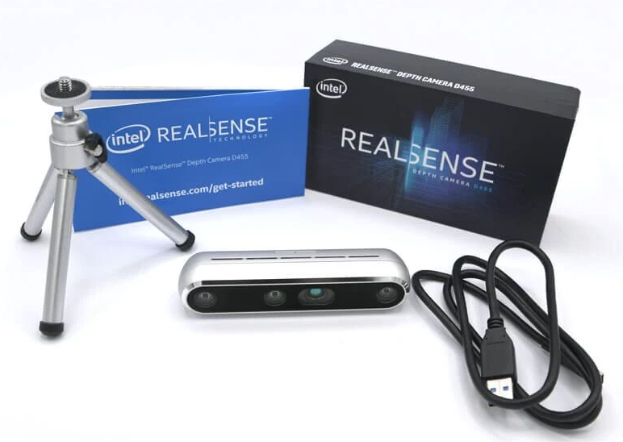
\includegraphics[width=0.55\linewidth]{images/COLMAP/D455_device.png}
\caption{Intel RealSense D455 Depth Camera.}
\label{fig:realsense}
\end{center}
 \end{figure}

 \section{Requirements} 

This lab requires Python 3.8+. You \textbf{must} create a virtual environment to manage hardware-specific libraries. The RealSense SDK (\texttt{pyrealsense2}) is highly sensitive to binary compatibility; using a \texttt{venv} prevents conflicts with system-level packages (see the next section for venv).

%\noindent \texttt{python -m venv rs\_env}\\ 
%\noindent \texttt{rs\_env\textbackslash Scripts\textbackslash activate \# (Windows)}\\ 
%\noindent \texttt{pip install pyrealsense2 opencv-python numpy}\


\noindent Note: Ensure your computer is equipped with a USB 3.0/3.1 port. A USB 2.0 port will severely limit resolution and framerate.


\section{Activities}

%\subsection*{Activity 0: Setting up the Camera and Virtual Environment}

%\begin{itemize} \item Objective: Isolate the development environment and verify hardware communication via the RealSense SDK. 
%\item Instructions: 
%\begin{itemize} 
%\item Connect the D455 to a USB 3.0 port. 
%\item Create and activate your \texttt{rs\_env} as described in the Requirements section. 
%\item Open the \textbf{RealSense Viewer} to check the firmware version. If prompted, update the firmware to ensure sensor calibration is accurate. \end{itemize} \end{itemize}


\subsection*{Activity 0: Basic Connectivity and Environment Setup}

\begin{itemize}
\item \textbf{Objective:} Establish communication with the Intel RealSense D455 and isolate the development environment to ensure library compatibility.
\item \textbf{Instructions:}
\begin{itemize}
\item \textbf{Step 1: Driver and SDK Installation}
    \begin{itemize}
    \item \textbf{Windows:} Download the latest \texttt{Intel.RealSense.SDK-Win10.exe} from the Official GitHub Releases: \href{https://github.com/IntelRealSense/librealsense/releases/latest}{https://github.com/IntelRealSense/librealsense/releases/latest}. Run the installer to set up the RealSense Viewer and USB drivers.
    \item \textbf{Ubuntu:} Register the Intel repository and install via \texttt{apt} using the following commands:
    \begin{verbatim}
    sudo apt install librealsense2-dkms librealsense2-utils 
    sudo apt install librealsense2-dev librealsense2-dbg
    \end{verbatim}
    \end{itemize}
\item \textbf{Step 2: Firmware Verification} 
    Launch the \texttt{RealSense Viewer}. If a "Firmware Update Available" notification appears in the top-right corner, proceed with the update to ensure the D455's global shutter and IMU are properly calibrated.
\item \textbf{Step 3: Virtual Environment Setup}
    Open your project folder and initialize the Python environment:
    \begin{verbatim}
    python -m venv rs_env
    source rs_env/bin/activate  # Linux/Mac
    rs_env\Scripts\activate     # Windows
    pip install pyrealsense2 opencv-python numpy
    \end{verbatim}
\end{itemize} 
\end{itemize}
\vspace{-3 mm}
Once the viewer is installed, run it (see Fig.~\ref{fig:viewer}). Explore the 2D and 3D options, see the top right corner.
 \begin{figure}[b!]
\begin{center}
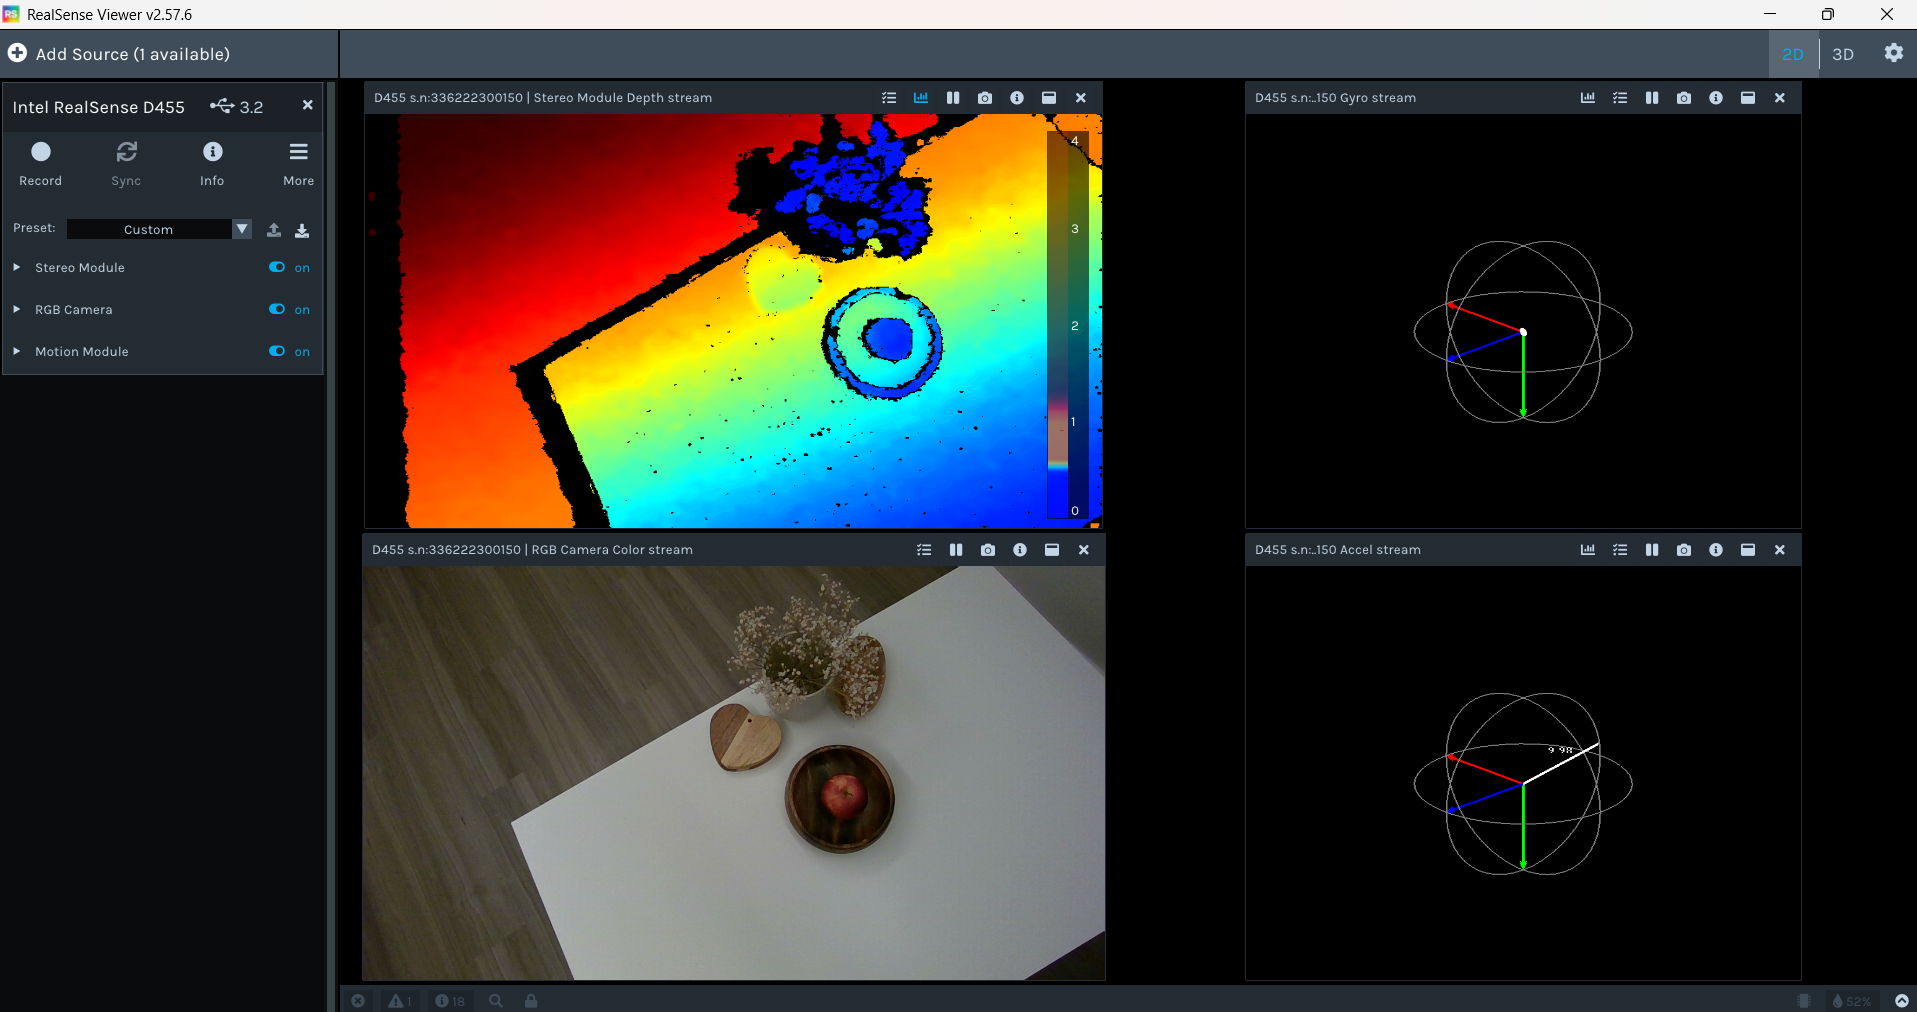
\includegraphics[width=.79\linewidth]{images/COLMAP/D455_viewer.png}
\caption{Intel D455 viewer.}
\label{fig:viewer}
\end{center}
 \end{figure}


\newpage
\subsection*{Activity 1: Real-Time Aligned Data Logging}

\begin{itemize} \item Objective: Capture synchronized RGB-D pairs where the depth map is aligned to the RGB camera's coordinate system. \item Instructions: \begin{itemize} \item Run the \texttt{d455\_logger.py} script. \item This script uses the \texttt{rs.align} object to mathematically project the depth data onto the RGB lens's viewpoint. \item Press \textbf{SPACE} to save a "Raw" frame. \end{itemize} \item Data Output: \begin{itemize} \item \texttt{.png}: Lossless RGB image. \item \texttt{.npy}: Raw 16-bit NumPy array containing depth in millimeters. \item \texttt{.csv}: Metadata log containing hardware exposure and gain values. \end{itemize} \end{itemize}


\subsection*{Activity 2: Data Playback and Quality Inspection}

\begin{itemize} 
\item Objective: Review the logged 3D data and verify that the RGB-Depth alignment is correct. 
\item Instructions: \begin{itemize} 
\item Run the \texttt{d455\_browser.py} script. 
\item Use \textbf{SPACE} to iterate through frames or \textbf{'c'} for continuous playback. 
\item Observe the "Depth Shadows", i.e. areas where the camera could not see (represented as black pixels). Ensure your target objects are not within these shadow regions. 
\end{itemize} 
\end{itemize}


\subsection*{Activity 3: Dataset Preparation for 3D Reconstruction (COLMAP)}

\begin{itemize} 
\item Objective: Export captured data for processing in an external Structure-from-Motion (SfM) pipeline. 
\item Instructions: \begin{itemize} 
\item Isolate the \texttt{.png} files into an \texttt{/images} directory. 
\item Load the directory into \textbf{COLMAP}. 
\item Perform Feature Extraction and Sequential Matching. 
\item Because the D455 uses a global shutter, features will remain sharp even if the camera was moving during capture, resulting in a higher-quality 3D point cloud. 
\item Try two sets of data: a small scale from a desktop object, a large scale environment, e.g. a room-sized environment.
\end{itemize} 
\end{itemize}

\end{document}
